\section{Solução desenvolvida}
\label{sec:iotGateway}

Além deste artigo, foi desenvolvida uma solução de software de Smart IoT Gateway que está disponibilizada no Github \cite{IoTGatewayGithub}. Esta seção propõe a detalhar os objetivos e decisões arquiteturais. Sendo assim, desenvolveu-se uma solução de Smart IoT Gateway, capaz de receber dados através de uma rede utilizando o protocolo MQTT, armazenar os dados recebidos e com em um cadastro prévio do dispositivo, os dados recebidos devem embasar uma análise que definirá a execução ou não  de um fluxo de notificação através de SMS para um número definido.

\subsection{Tecnologias} 
\begin{itemize}
	\item Node.js v6.x \cite{NodeJS};
	\item TypeScript 2.3 com transpile para ES6 \cite{Typescript};
	\item TSLint 4.x com recomendações gerais padrão \cite{TSLint};
	\item Jest para teste unitário e cobertura \cite{Jest};
	\item Angular 1.6 para o front end da aplicação \cite{AngularJS};
	\item MongoDB \cite{MongoDB}.
\end{itemize}

O Node.js foi escolhido por conta de seu baixo consumo de memória e processamento, além da sua característica de Non-Blocking IO, garantindo que possamos servir mais clientes com menos recursos, objetivo essencial para aplicações que podem ser executadas em um Raspberry Pi por exemplo. A escolha pelo TypeScript, linguagem que é um superset do Javascript padrão foi motivada por garantir uma estrutura tipada, de forma que a manutenção do código fosse facilitada e as regras de negócio pudessem estar ligadas a um contrato de objeto. Já o angular 1 foi escolhido, por ser uma tecnologia que funciona com javascript nativo, sem necessidade de nenhum pós-processador para servir a aplicação aos clientes, permitindo o seu uso diretamente entre os arquivos estáticos do mesmo servidor Node.js que expõe a aplicação. Além disso, contou como um ponto para a escolha, a experiência prévia da equipe no desenvolvimento com esta tecnologia.

\subsection{Modelo de Dados} 
O modelo de dados foi concebido com a intenção de tornar as etapas do processo altamente plugáveis e customizáveis no curto e longo prazo, garantindo as funcionalidades básicas do MVP executado e a possibilidade de extensibilidade no futuro com retrocompatibilidade.
A modelagem desenvolve uma estrutura sequencial que parte da identificação do dispositivo, análise dos gatilhos ligados a este dispositivo, avaliação da operação lógica e liberação para execução do evento, ver Figura~\ref{fig:modeloDeDados}. Outras entidades não ligadas aos processo principal, visam dar suporte estas operações entregando configurações do sistema e registro de históricos para análise futura. 

\begin{figure}[h!]
	\begin{center}
		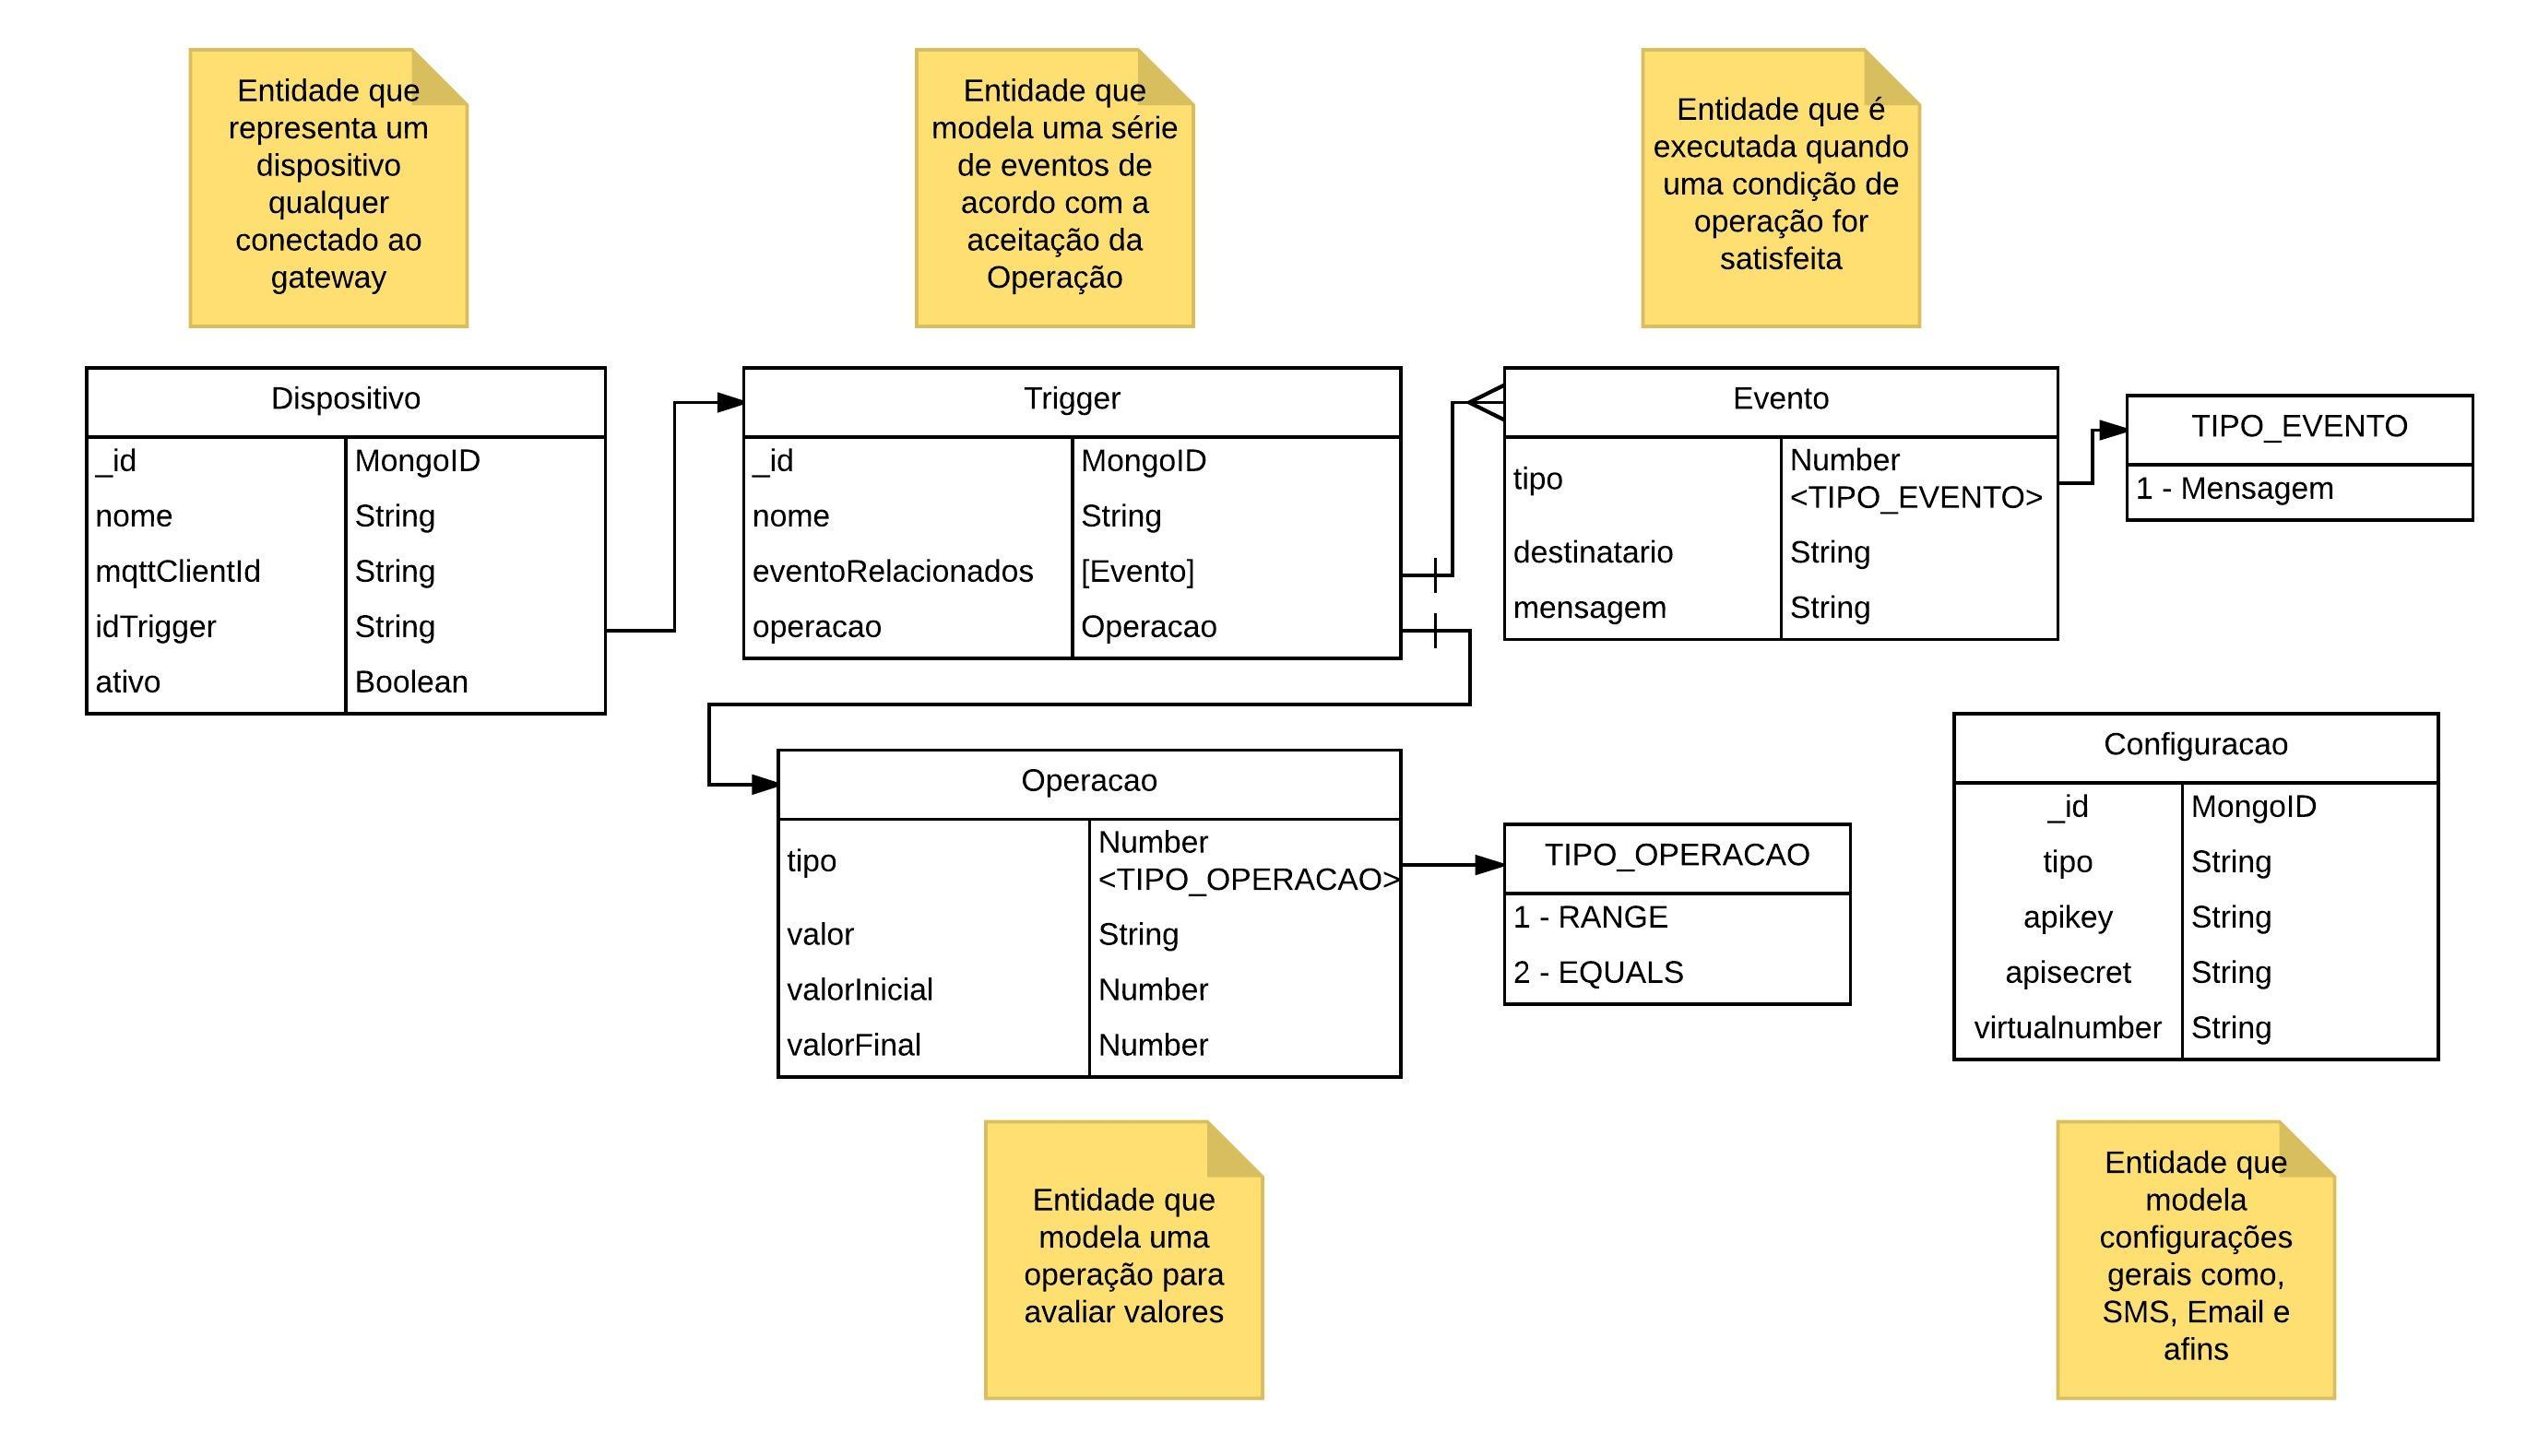
\includegraphics[width=1\textwidth]{./img/modelo-de-dados}
		\caption{Modelo de dados.}
		\label{fig:modeloDeDados}
	\end{center}
\end{figure}
